\documentclass[a4paper,12pt]{article}
\usepackage[utf8]{inputenc}
\usepackage[T1]{fontenc}
\usepackage[brazil]{babel}
\usepackage{lmodern}
\usepackage[margin=2.5cm]{geometry}
\usepackage{amsmath,booktabs,graphicx}
\usepackage{microtype,caption,placeins,float}
\usepackage[hidelinks]{hyperref}
\graphicspath{{images/}}
\captionsetup{font=small,labelfont=normalfont}
\setlength{\textfloatsep}{12pt plus 2pt minus 2pt}
\setlength{\intextsep}{10pt plus 2pt minus 2pt}
\setlength{\parskip}{1pt}
\setlength{\emergencystretch}{1em}
\hypersetup{pdftitle={Visão Computacional TA02 - Calibração},
  pdfsubject={Relatório de Visão Computacional},pdflang={pt-BR}}

% Edit the two author names and repository URL before submission.
\title{\Large Visão Computacional TA02 - Calibração}
\author{Marcelo Gyovani Pereira \and Vinícius Evair da Silva}
\date{}

\begin{document}
\maketitle
\vspace{-1.5em}
\begin{center}
  \small Repositório:
  \url{https://github.com/marzelop/visao-ta02/}
\end{center}

\section{Introdução}

A calibração de uma câmera estima os parâmetros que relacionam pontos de uma
cena às suas posições na imagem. A matriz intrínseca reúne as distâncias focais
em pixels e o ponto principal; os coeficientes de distorção representam desvios
em relação ao modelo de projeção ideal. Esses parâmetros permitem corrigir
deformações geométricas e projetar pontos tridimensionais em coordenadas de
imagem, conforme os procedimentos do OpenCV~\cite{opencv-tutorial,opencv-calib3d}.

Neste trabalho, foram calibradas duas câmeras de um smartphone. Os parâmetros
obtidos foram aplicados à correção de fotografias de teste e à projeção de
pontos de um tabuleiro. O principal experimento quantitativo utiliza novas
fotografias, não incluídas na calibração, e compara posições observadas e
previstas de quatro cantos reservados da estimação da pose em cada imagem.

\section{Metodologia}

Foram utilizadas as câmeras principal, no modo 1x (\texttt{cam1}), e ultrawide,
no modo 0,5x (\texttt{cam05}), de um Samsung Galaxy A56. A coleta inicial reuniu
22 fotografias do tabuleiro por câmera, com resolução de $2992\times2992$ pixels,
variando posição, distância e inclinação do padrão. O tabuleiro possui
$5\times5$ quadrados de lado $3{,}1$~cm e $4\times4$ cantos internos. Os dados
foram organizados em diretórios independentes para cada câmera.
Para avaliar a projeção, foram obtidas outras três fotografias do tabuleiro por
câmera, armazenadas em \texttt{project\_test/} e mantidas fora da calibração.

A implementação utiliza Python, NumPy e OpenCV. Em \texttt{calibrate.py}, os
cantos são detectados com \texttt{cv2.findChessboardCorners()}, com
\texttt{cv2.findChessboardCornersSB()} como alternativa em caso de falha, e
refinados por \texttt{cv2.cornerSubPix()}. O refinamento utiliza janela de
$11\times11$ pixels, limite de 30 iterações e tolerância de $0{,}001$ pixel.
A Figura~\ref{fig:corners} apresenta uma detecção existente no repositório.

A calibração utiliza \texttt{cv2.calibrateCamera()}, que recebe as coordenadas
do padrão e as observações 2D. Em seguida, \texttt{undistort.py} aplica
\texttt{cv2.undistort()} às fotografias, enquanto \texttt{project.py} estima
a pose com \texttt{cv2.solvePnP()} e calcula projeções com
\texttt{cv2.projectPoints()}. Todos os cálculos utilizam a resolução original;
os detalhes ampliados nas figuras servem apenas à apresentação.

\begin{figure}[H]
  \centering
  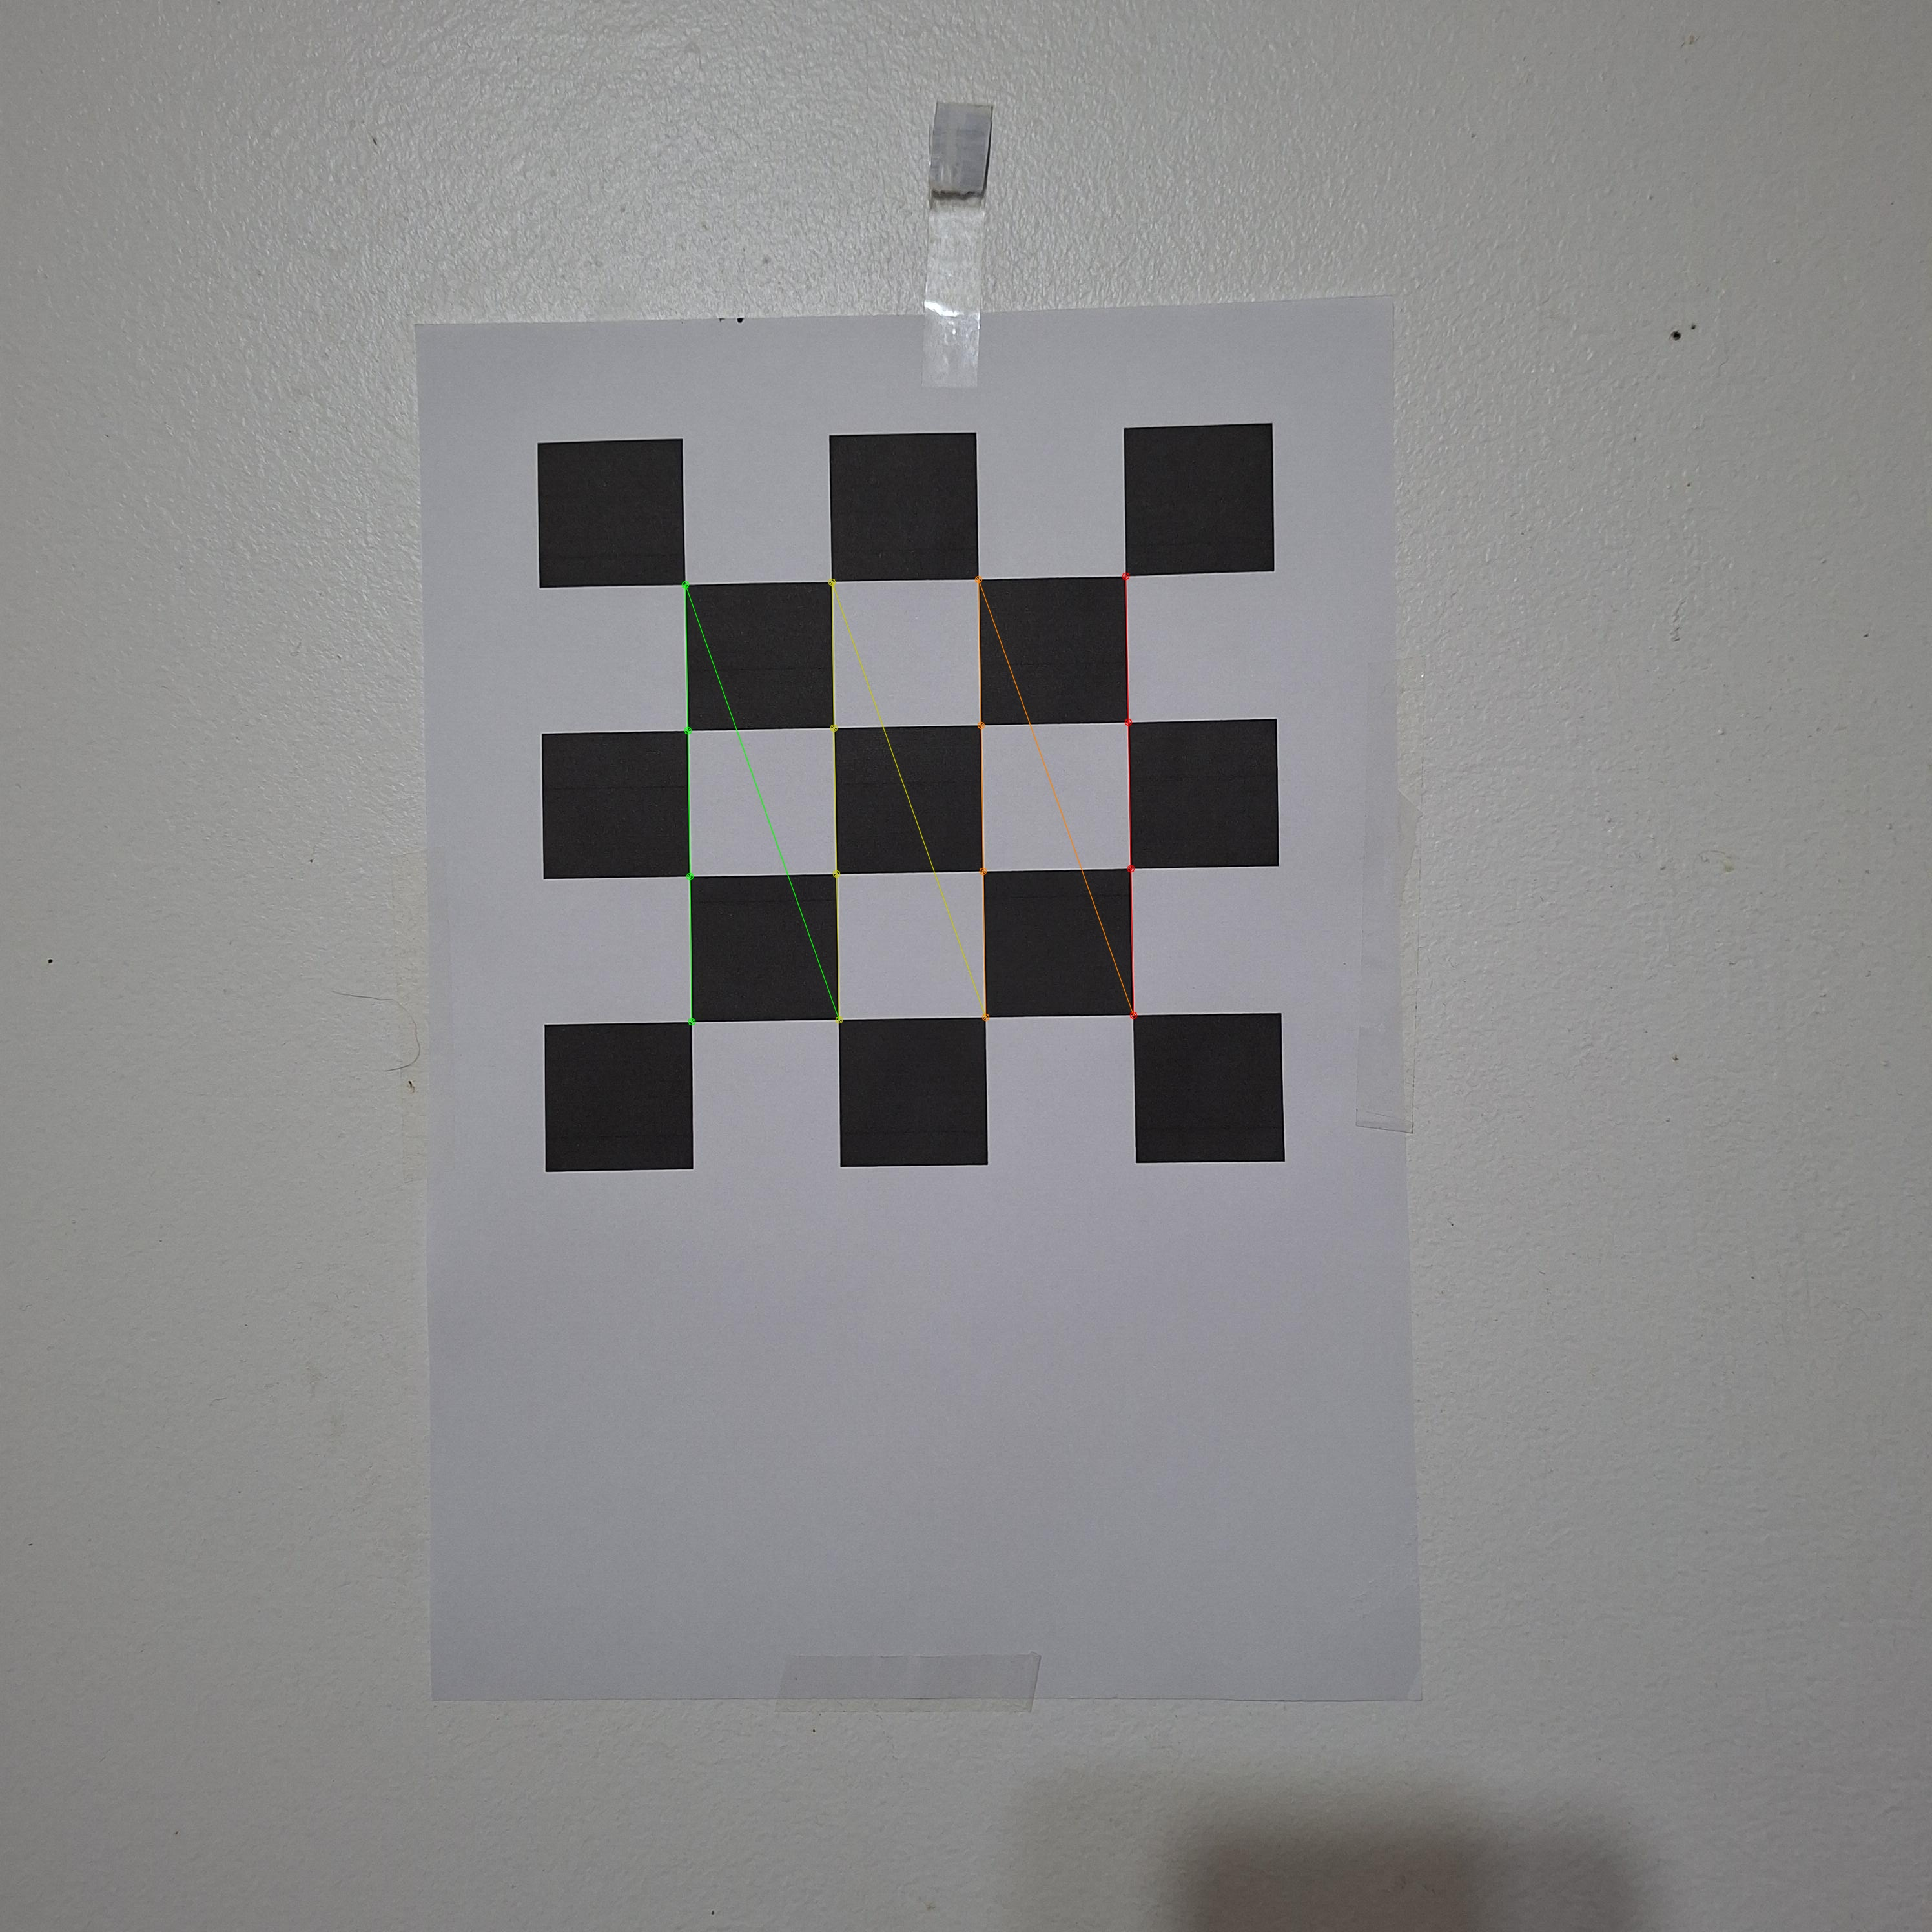
\includegraphics[width=0.39\linewidth,trim=650bp 942bp 792bp 480bp,clip]{board-corners.jpg}
  \caption{Detalhe da fotografia \texttt{001.jpg} da câmera 1x, com os 16 cantos
  internos detectados e conectados pelo OpenCV.}
  \label{fig:corners}
\end{figure}

\FloatBarrier
\section{Calibração das câmeras}

A calibração final utilizou 22 fotografias da câmera 1x e 20 da câmera 0,5x.
Conforme o histórico experimental informado, a primeira calibração da câmera
0,5x empregou as 22 fotografias; as imagens 019 e 022 apresentaram
os maiores erros individuais e foram retiradas manualmente. Após essa seleção,
o RMS passou de aproximadamente $1{,}686$ para $1{,}463$ pixel. Os arquivos
atuais registram o ajuste final com 20 imagens, sem novos descartes na execução.

Os arquivos \texttt{calibration.npz} e \texttt{log.txt}, nos diretórios de cada
câmera, registram os mesmos parâmetros. As matrizes intrínsecas, em pixels, são
\begin{equation}
K_{1\mathrm{x}}=
\begin{bmatrix}
2715{,}936 & 0 & 1484{,}581\\
0 & 2706{,}305 & 1520{,}002\\
0 & 0 & 1
\end{bmatrix},
\label{eq:k1}
\end{equation}
\begin{equation}
K_{0{,}5\mathrm{x}}=
\begin{bmatrix}
1600{,}726 & 0 & 1586{,}526\\
0 & 1596{,}602 & 1494{,}484\\
0 & 0 & 1
\end{bmatrix}.
\label{eq:k05}
\end{equation}
As menores distâncias focais em pixels da câmera 0,5x são compatíveis com seu
enquadramento mais amplo; não representam medidas físicas em milímetros.

\begin{table}[H]
  \centering
  \caption{Resultados do ajuste final. Os erros são expressos em pixels.}
  \label{tab:calibration}
  \begin{tabular}{lrrr}
    \toprule
    Câmera & Imagens & RMS & Erro médio euclidiano\\
    \midrule
    Principal (1x) & 22 & 0,910 & 0,667\\
    Ultrawide (0,5x) & 20 & 1,463 & 1,168\\
    \bottomrule
  \end{tabular}
\end{table}

A Tabela~\ref{tab:distortion} apresenta os coeficientes adimensionais na
convenção do OpenCV: $k_1$, $k_2$ e $k_3$ são radiais; $p_1$ e $p_2$ são
tangenciais. A notação científica mantém visíveis os coeficientes de menor
magnitude.
\begin{table}[H]
  \centering
  \caption{Coeficientes de distorção das duas câmeras.}
  \label{tab:distortion}
  \begin{tabular}{lrr}
    \toprule
    Coeficiente & Principal (1x) & Ultra-angular (0,5x)\\
    \midrule
    $k_1$ & $1{,}041\times10^{-1}$ & $-1{,}245\times10^{-2}$\\
    $k_2$ & $-3{,}006\times10^{-1}$ & $3{,}508\times10^{-2}$\\
    $k_3$ & $9{,}202\times10^{-5}$ & $1{,}756\times10^{-2}$\\
    $p_1$ & $2{,}460\times10^{-3}$ & $8{,}152\times10^{-4}$\\
    $p_2$ & $1{,}630\times10^{-3}$ & $1{,}142\times10^{-2}$\\
    \bottomrule
  \end{tabular}
\end{table}

O RMS é a raiz da média das distâncias de reprojeção ao quadrado. O erro médio
é a média das distâncias euclidianas entre cantos detectados e reprojetados.
Com 16 pontos por imagem, a média das médias por imagem coincide com a global.

A câmera principal apresentou menor erro nas duas medidas da
Tabela~\ref{tab:calibration}. Campo de visão, tamanho do padrão na imagem,
localização dos cantos e adequação do modelo são possíveis fatores para essa
diferença, mas não foram isolados experimentalmente. Além disso, a redução do
RMS após retirar imagens da câmera 0,5x mede o ajuste ao conjunto selecionado.

\FloatBarrier
\section{Correção da distorção}

Os parâmetros de cada câmera foram reutilizados em \texttt{undistort.py} para
corrigir a distorção geométrica com \texttt{cv2.undistort()}. A função
\texttt{cv2.}\allowbreak\texttt{getOptimalNewCameraMatrix()} determina uma nova matriz
intrínseca para a mesma resolução, com duas escolhas de
$\alpha$~\cite{opencv-tutorial}. Para $\alpha=0$, prioriza-se uma região válida,
evitando bordas pretas e reduzindo o campo de visão. Para $\alpha=1$, preserva-se
mais do campo original, com possíveis regiões sem pixels correspondentes,
representadas em preto. O programa não recorta a região de interesse retornada
nem redimensiona os arquivos corrigidos.

Foram utilizadas fotografias de teste sem tabuleiro, separadas das imagens de
calibração. As Figuras~\ref{fig:undistort1} e~\ref{fig:undistort05} reproduzem
comparações já geradas para \texttt{fogao1.jpg}. As bordas da porta e os rejuntes
dos azulejos, próximos aos limites das fotografias, permitem inspecionar
visualmente as alterações. Cada câmera observa a cena com enquadramento próprio;
a comparação relevante ocorre entre as versões da mesma fotografia.

\begin{figure}[H]
  \centering
  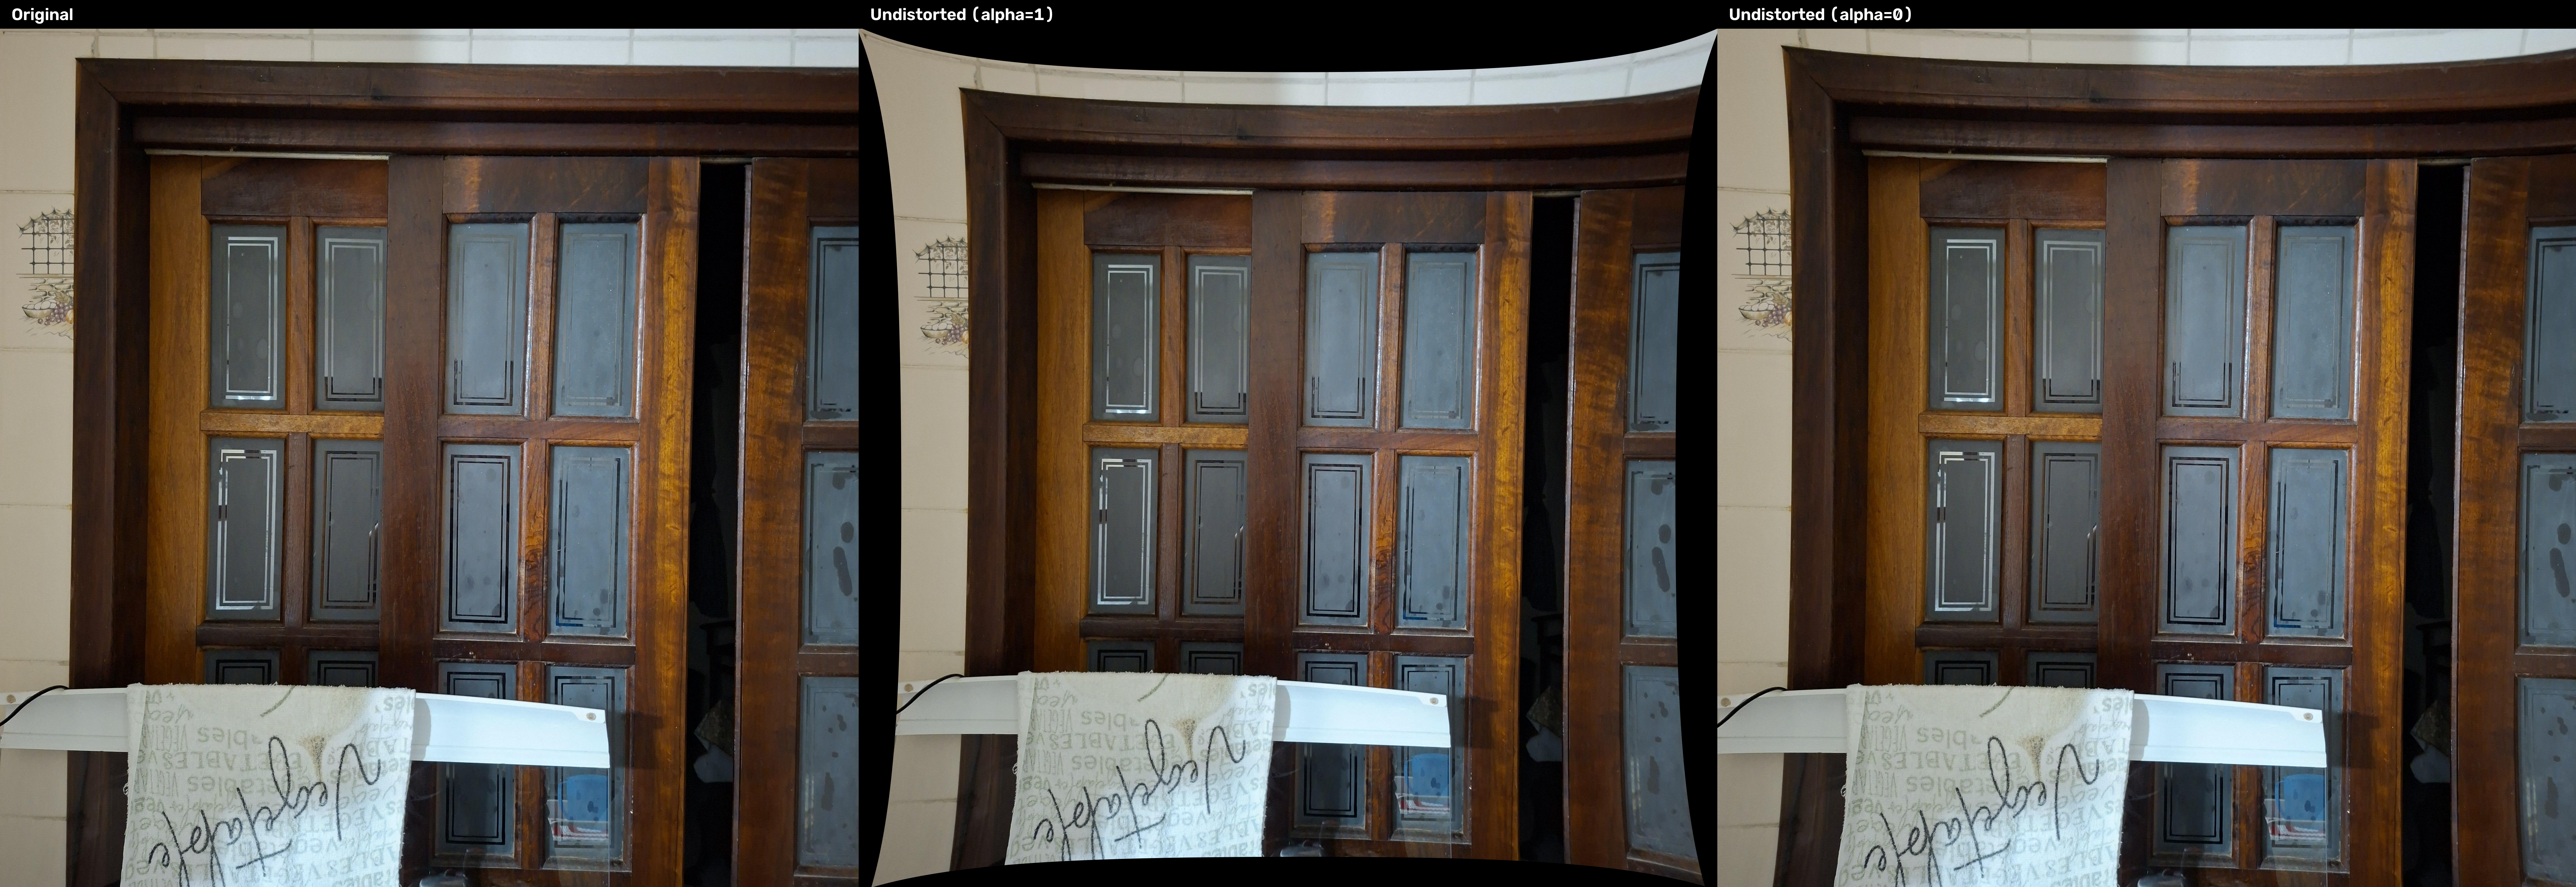
\includegraphics[width=\linewidth]{undistortion-cam1.jpg}
  \caption{Câmera principal (1x), fotografia de teste \texttt{fogao1.jpg}.
  Da esquerda para a direita: original, corrigida com $\alpha=1$ e corrigida
  com $\alpha=0$. A faixa preta curva na versão central corresponde a regiões
  sem amostras da imagem original.}
  \label{fig:undistort1}
\end{figure}

\begin{figure}[H]
  \centering
  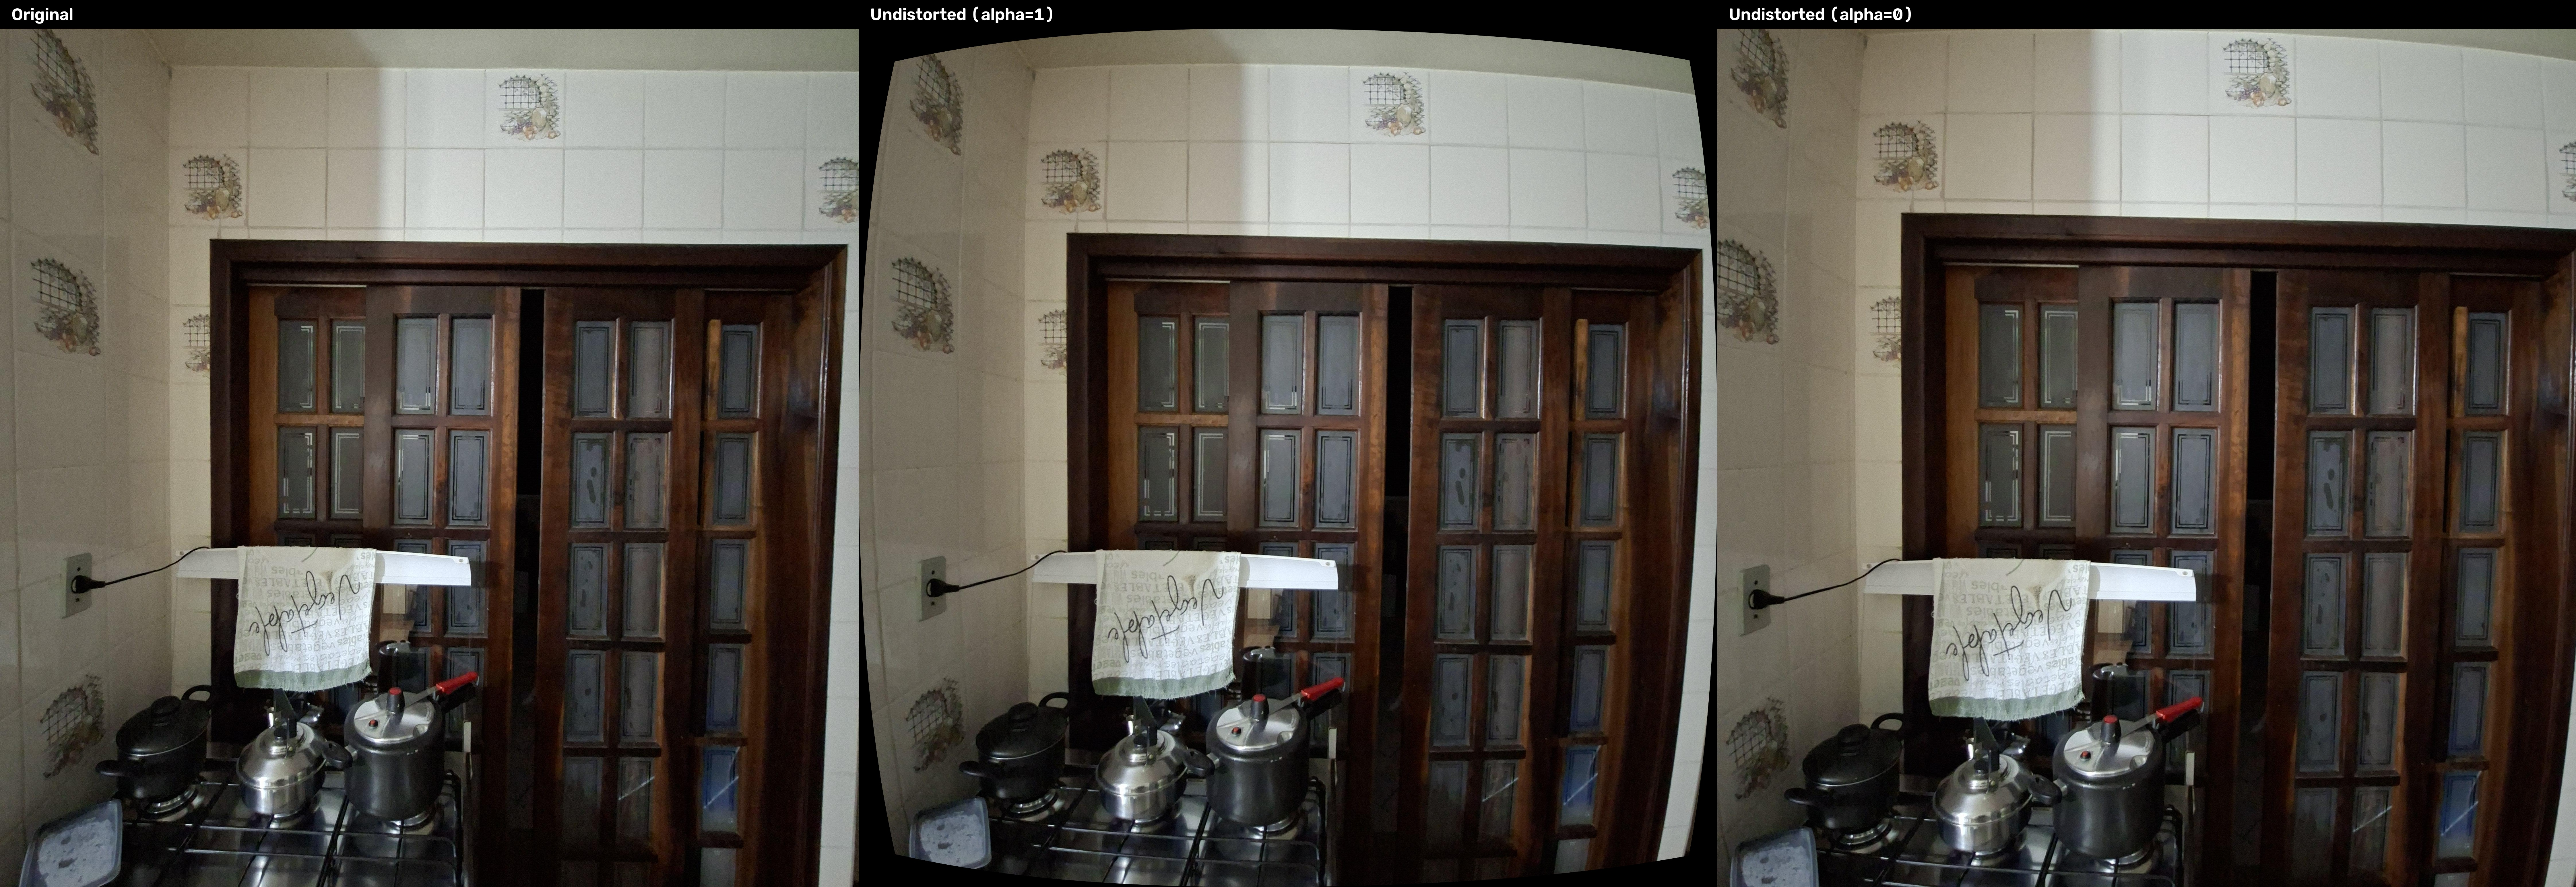
\includegraphics[width=\linewidth]{undistortion-cam05.jpg}
  \caption{Câmera ultrawide (0,5x), fotografia de teste \texttt{fogao1.jpg}.
  A ordem é original, $\alpha=1$ e $\alpha=0$. Observam-se o remapeamento da
  cena, as bordas sem correspondência e a mudança de enquadramento.}
  \label{fig:undistort05}
\end{figure}

As diferenças locais podem ser discretas, embora a alteração de enquadramento
seja visível. Não foi medida a retidão das linhas ou outra métrica geométrica
nas imagens de teste; portanto, essas figuras não demonstram uma melhoria
quantitativa da geometria. A correção também não elimina efeitos de
perspectiva, como a convergência de linhas associada à orientação da câmera em
relação à cena. Bordas pretas, por sua vez, decorrem do domínio do remapeamento
e não representam regiões adicionais capturadas pela câmera.

\FloatBarrier
\section{Projeção de pontos 3D em imagens 2D}

\subsection{Estimação da pose e separação dos pontos}

O experimento de \texttt{project.py} utiliza os parâmetros já salvos e três
fotografias inéditas por câmera, de \texttt{project\_test/}, sem recalibrar as
câmeras. O mesmo procedimento é aplicado às fotografias da calibração para
comparação. Os 16 cantos do tabuleiro têm coordenadas conhecidas
$\mathbf{P}_{r,c}=(3{,}1c,\,3{,}1r,\,0)$~cm, com $r,c\in\{0,1,2,3\}$.
O índice é $4r+c$, com a coluna variando primeiro, conforme a ordenação usada
na calibração. A origem está no canto de índice zero. Essas coordenadas
pertencem ao referencial local do tabuleiro, e não a um sistema global.

Após a detecção e o refinamento dos cantos, 12 correspondências entre pontos
3D e posições 2D observadas estimam a rotação e a translação do tabuleiro por
uma única chamada a \texttt{cv2.solvePnP()}, no modo
\texttt{SOLVEPNP\_ITERATIVE}. A pose transforma o referencial do tabuleiro no
referencial da câmera~\cite{opencv-calib3d}. A seleção é determinística: os
índices $0$, $3$, $12$ e $15$, situados nos quatro extremos da grade interna,
ficam reservados; os outros 12 se distribuem pelas quatro linhas e colunas.
Os pontos reservados não entram no \texttt{solvePnP()} nem em um refinamento
posterior da pose.

Com a pose estimada, \texttt{cv2.projectPoints()} calcula as coordenadas previstas
dos quatro pontos reservados, usando a matriz intrínseca, os coeficientes de
distorção e os vetores de rotação e translação. A comparação é feita no domínio
da fotografia original: não são usadas as imagens corrigidas por
\texttt{undistort.py}, pois a projeção já incorpora a distorção. O procedimento
é repetido por fotografia, com 12 pontos de pose e quatro de validação.

\subsection{Métricas e resultados}

Se $(u_i,v_i)$ é a posição observada e $(\hat{u}_i,\hat{v}_i)$ a posição
prevista, o erro individual, em pixels, é
\begin{equation}
e_i=\sqrt{(u_i-\hat{u}_i)^2+(v_i-\hat{v}_i)^2}.
\label{eq:error}
\end{equation}
Para os $N$ pontos de validação de uma câmera, calculam-se
\begin{equation}
\bar e=\frac{1}{N}\sum_{i=1}^{N}e_i,\qquad
\mathrm{RMSE}=\sqrt{\frac{1}{N}\sum_{i=1}^{N}e_i^2},\qquad
e_{\max}=\max_i e_i.
\label{eq:metrics}
\end{equation}
A média descreve o desvio típico, o RMSE atribui maior peso aos erros elevados
e o máximo registra o maior desvio individual. Todas as métricas globais
utilizam os erros ponto a ponto; não se faz a média dos RMSEs por imagem.

As três fotografias inéditas de cada câmera foram processadas sem falhas de
detecção ou estimação da pose, totalizando 12 pontos de validação por câmera.
Os resultados estão em \texttt{projections/tests/summary.txt} e
\texttt{points.csv}. A Tabela~\ref{tab:projection} também apresenta a referência
obtida nas 22 fotografias de calibração da câmera 1x e nas 20 da câmera 0,5x,
com 88 e 80 pontos reservados, respectivamente. As métricas de cada conjunto
foram calculadas separadamente, sem excluir erros elevados.

\begin{table}[H]
  \centering
  \caption{Erros de projeção em pixels: fotografias da calibração e teste inédito.}
  \label{tab:projection}
  \begin{tabular}{llrrrr}
    \toprule
    Câmera & Conjunto & Imagens & Média & RMSE & Máximo\\
    \midrule
    1x & Calibração & 22 & 1,121 & 1,575 & 5,121\\
    1x & Teste inédito & 3 & 2,839 & 4,061 & 9,162\\
    \midrule
    0,5x & Calibração & 20 & 2,112 & 2,563 & 6,119\\
    0,5x & Teste inédito & 3 & 2,418 & 3,060 & 6,821\\
    \bottomrule
  \end{tabular}
\end{table}

As Figuras~\ref{fig:projection1} e~\ref{fig:projection05} apresentam fotografias
inéditas das duas câmeras, com detalhe da região do tabuleiro. Os marcadores
são maiores apenas para facilitar a leitura; as distâncias da
Equação~\eqref{eq:error} foram calculadas com coordenadas de subpixel. Como os
desvios são pequenos na escala das figuras, observações e projeções podem
aparecer quase sobrepostas.

\begin{figure}[H]
  \centering
  \captionsetup{justification=raggedright,singlelinecheck=false}
  \begin{minipage}[t]{0.48\linewidth}
  \centering
  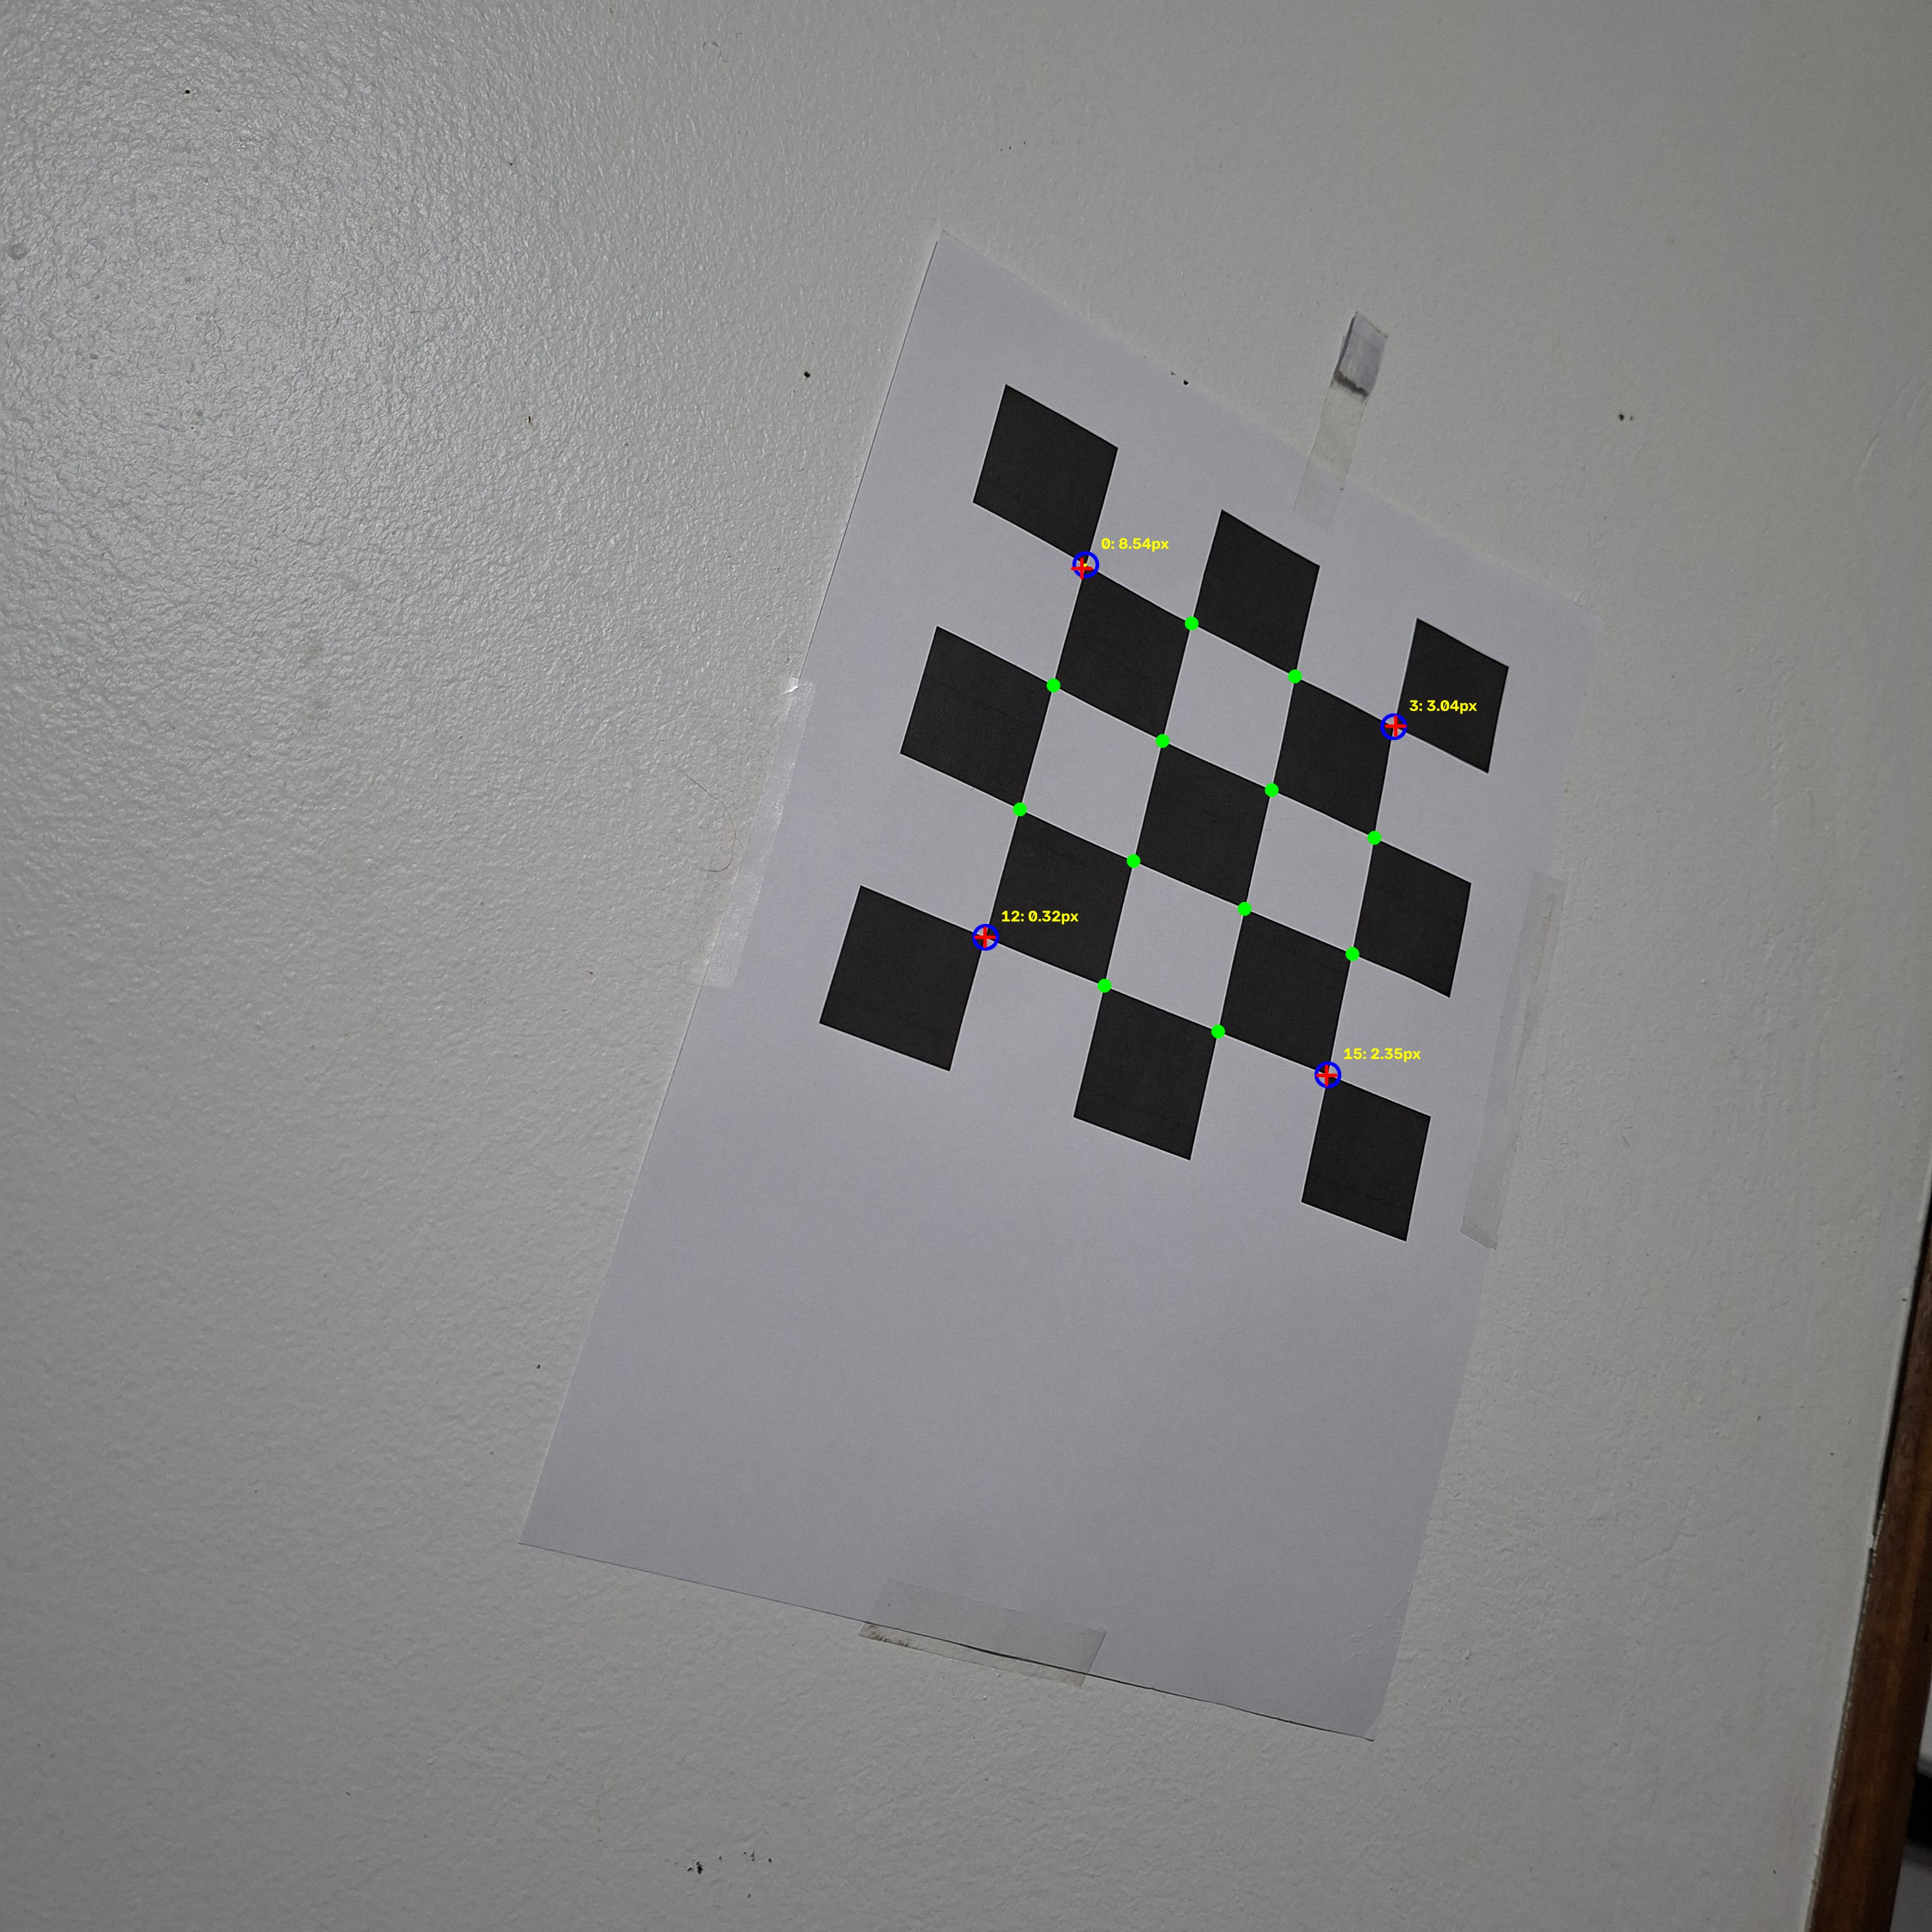
\includegraphics[height=5.5cm,trim=1325bp 1078bp 584bp 674bp,clip]{projection-cam1.jpg}
  \caption{Câmera 1x, fotografia inédita \texttt{001.jpg}. Verde: pose;
  azul: observações reservadas; vermelho: projeções. Amarelo: conexões e
  rótulos de erro. Média nesta imagem: $3{,}562$~px.}
  \label{fig:projection1}
  \end{minipage}\hfill
  \begin{minipage}[t]{0.48\linewidth}
  \centering
  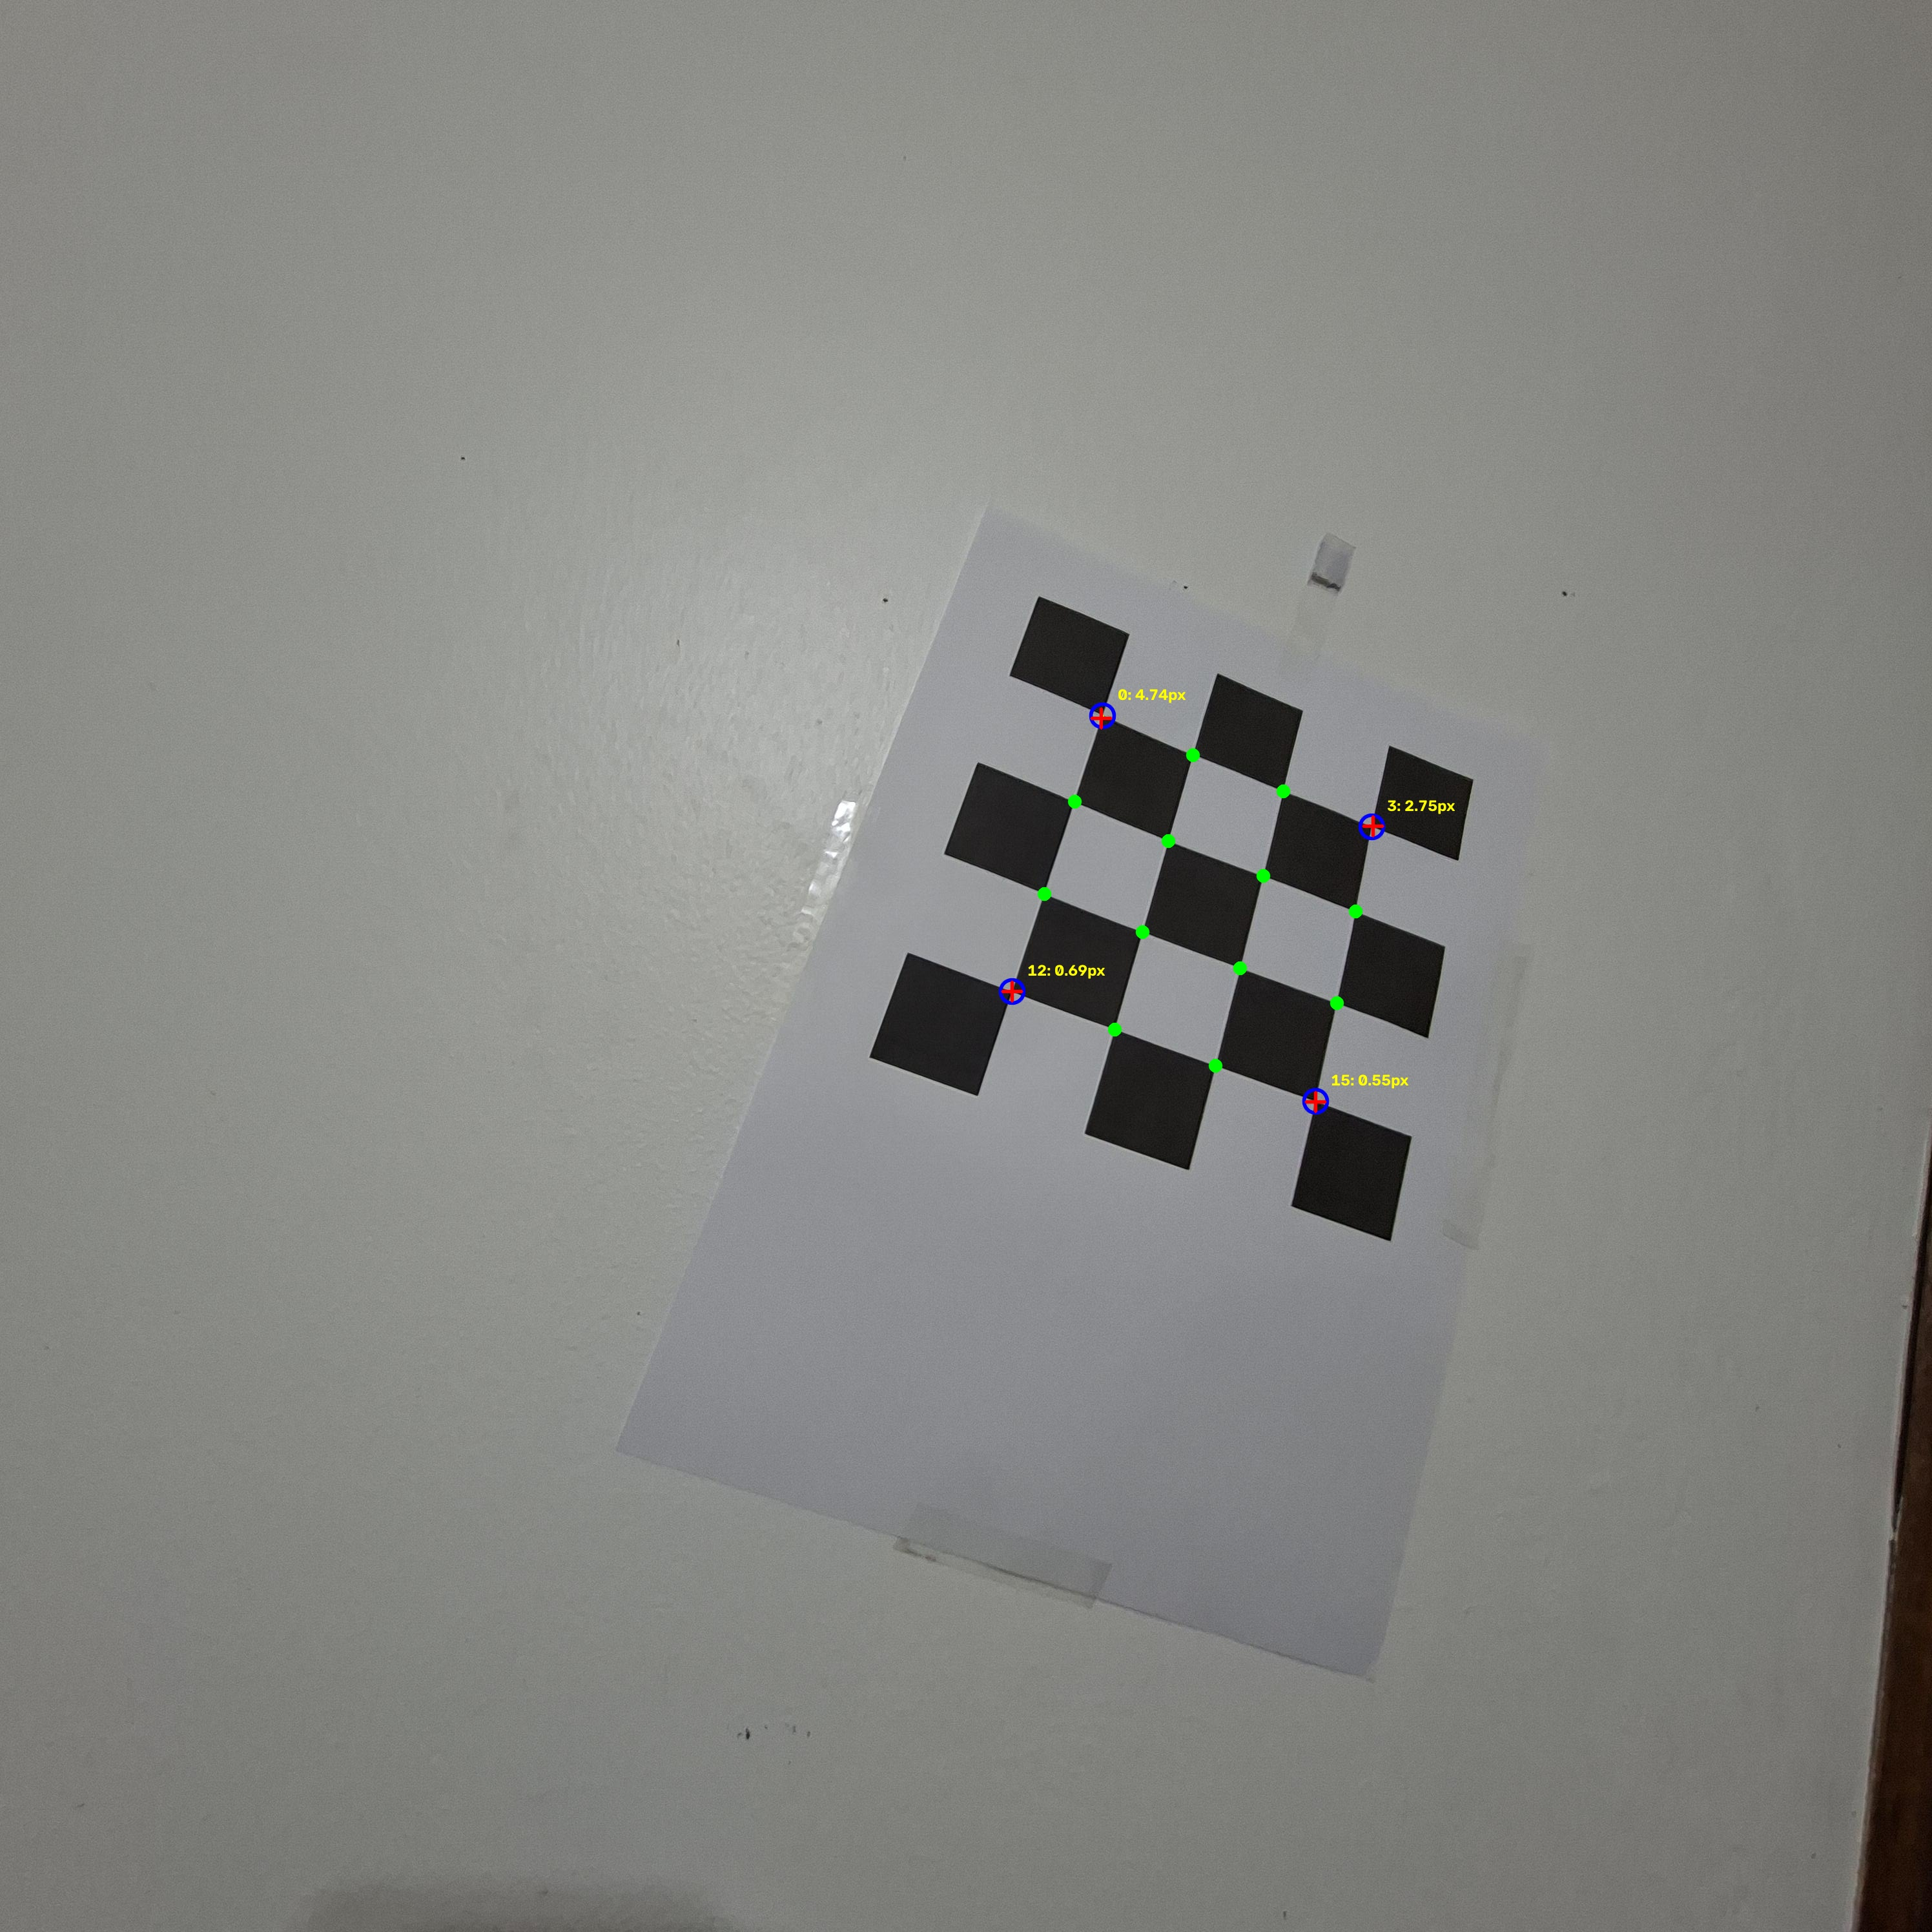
\includegraphics[height=5.5cm,trim=1367bp 1037bp 619bp 907bp,clip]{projection-cam05.jpg}
  \caption{Câmera 0,5x, fotografia inédita \texttt{002.jpg}, com a convenção da
  Figura~\ref{fig:projection1}. Média nesta imagem: $2{,}183$~px.
  As duas figuras foram enquadradas somente no documento.}
  \label{fig:projection05}
  \end{minipage}
\end{figure}

\FloatBarrier
Nas fotografias inéditas, o erro médio aumentou $153{,}19\%$ na câmera 1x
e $14{,}50\%$ na câmera 0,5x; o RMSE aumentou $157{,}75\%$ e $19{,}41\%$,
respectivamente. A câmera 0,5x apresentou menores erros nesse novo conjunto,
embora a câmera principal tivesse menores erros nas fotografias da calibração.
A escala e a posição do tabuleiro, sua inclinação e resíduos do modelo podem
influenciar a diferença; esses fatores não foram isolados.

As novas fotografias não participaram da calibração intrínseca, e os quatro
cantos reservados também não participaram da estimação da pose. A avaliação
verifica, portanto, a projeção em imagens inéditas, mas a pose de cada imagem
continua sendo estimada a partir de 12 correspondências conhecidas. Com apenas
três imagens por câmera, os resultados descrevem esta amostra e não estabelecem
uma superioridade geral de uma das câmeras.

\FloatBarrier
\section{Conclusão}

A calibração foi realizada para as câmeras principal e ultrawide do
smartphone, obtendo-se matrizes intrínsecas e coeficientes de distorção que
foram reutilizados na correção de fotografias. Na validação da projeção
3D--2D em três fotografias inéditas por câmera, os erros médios foram
aproximadamente $2{,}84$ pixels para a câmera 1x e $2{,}42$ pixels para a câmera
0,5x. Os erros aumentaram em relação às fotografias da calibração, sobretudo
na câmera principal. Esta manteve os menores erros de calibração, enquanto
a câmera 0,5x apresentou menores erros de projeção na nova amostra.

As conclusões são limitadas pelo tamanho e pela seleção dos conjuntos, pelo
uso de um padrão plano e pelo número reduzido de fotografias inéditas.
A pose depende de correspondências 2D conhecidas em cada imagem, e a correção
das fotografias de teste foi examinada apenas visualmente. Um conjunto de teste
mais amplo, com condições de captura controladas e medidas de geometria,
permitiria avaliar melhor a generalização dos parâmetros.


\begin{thebibliography}{9}
\small
\bibitem{opencv-tutorial}
OPENCV. \textit{Camera Calibration}. OpenCV-Python Tutorials.
Disponível em:
\url{https://docs.opencv.org/4.x/dc/dbb/tutorial_py_calibration.html}.
Acesso em: 17 out. 2026.

\bibitem{opencv-calib3d}
OPENCV. \textit{Camera Calibration and 3D Reconstruction}.
Documentação do módulo calib3d. Disponível em:
\url{https://docs.opencv.org/4.x/d9/d0c/group__calib3d.html}.
Acesso em: 17 out. 2026.
\end{thebibliography}
\end{document}
